\chapter{Umsetzung}
\label{sec:Umsetzung}
Die in Kapitel \ref{sec:Grundlagen} beschriebenen Prozesse werden von dem Beispielstartup Agrishare durchlaufen. Zuerst wird die Anwendung von \textit{The Innovator's Method} beschrieben, welche in Abschnitt \ref{sec:TheInnovatorsMethod} eingehend erklärt ist. Basierend darauf führt das Agrishare-Team einen Sprint durch, welcher in Abschnitt \ref{sec:Sprint-Grundlagen} grundlegend beschrieben wird. Außerdem werden Methoden des \ac{TLS} Gesamtkonzeptes angewandt, welche in Abschnitt \ref{sec:LeanStartup} erläutert sind. Als Ergebnis daraus wird in Abschnitt \ref{BMC_Agrishare} das in \ref{BMC_Kapitel} eingeführte Modell des \ac{BMC} dargestellt. Die Beschreibung der von Agrishare umgesetzten Prozesse ist im Folgenden zusammengefasst geschildert.
\section{The Innovator's Method}

The Innovator's Method beschreibt eine Zusammenführung von etablierten Prozessen, um Schritt für Schritt ein erfolgreiches Startup aufzubauen.
Im Detail werden die Prozesse Sprint, The Lean Startup, sowie die Erstellung einer \ac{BMC} im Rahmen dieser Arbeit erklärt und umgesetzt.

\begin{figure}[h!]
	\begin{center}
		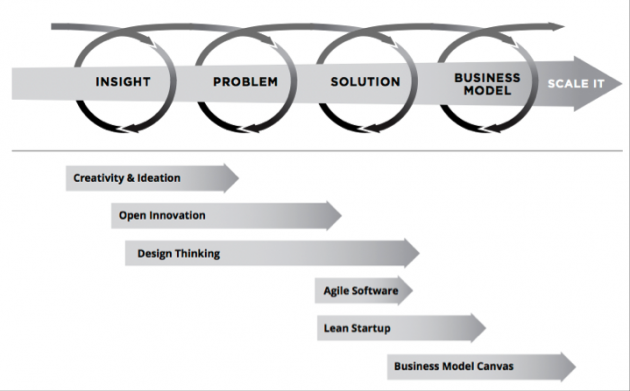
\includegraphics[width=\textwidth]{99_IMG/02_Grundlagen/innovatorsMethod.png}
		\caption{The Innovator's Method - Grundkonzept}
		\label{fig:TheInnovatorsMethod}
	\end{center}
\end{figure}

Allgemeiner gefasst, kann man The Innovator's Method in vier große Schritte aufteilen, wie in Abb. \ref{fig:TheInnovatorsMethod} dargestellt. Diese werden im Folgenden zusammengefasst erläutert.

\begin{enumerate}
	\item \textbf{Insight}
	
	In Schritt 1 liegt der Fokus darauf, die Zielgruppe zu beobachten, zu befragen und kennenzulernen. Erst wenn die Abläufe, welche die potentiellen Kunden zu durchlaufen haben, bekannt sind, kann daran angeknüpft werden. Nicht selten kommt es vor, dass überraschende Details erkannt werden, welche so ursprünglich nicht erwartet wurden. Das sind wesentliche Informationen, die ein kundenorientiertes Konzept ausmachen. Denn nur wenn alle Details über die kritische Ablauffolge klar sind, können daraus resultierende Probleme erkannt werden, wie im nächsten Punkt näher erklärt wird. 
	
	\item \textbf{Problem}
	
	Ein Problem kann hier auch ein Bedürfnis oder einen Wunsch erfüllen. Denn nicht immer löst ein neues Produkt ein bekanntes Problem. Meist werden daher Bedürfnisse erfüllt, von welchen der Nutzer ursprünglich nicht wusste, dass er sie hat. Um das herauszufinden, ist es essentiell, Schritt 1 so detailliert durchzuführen, dass diese Wünsche zum Vorschein kommen, ohne dass der Kunde sie formulieren muss. Das Problem per se muss dann gründlich herausgearbeitet werden, indem sich der Gründer in die Lage der Zielgruppe versetzt. Nur so ist es möglich, die entscheidenden Details, welche nicht auf den ersten Blick sichtbar sind, herauszufinden.
	
	\item \textbf{Solution}
	
	Die Lösung des vorher erarbeitetem und untersuchtem Problems soll nun prototypisiert werden. Im Vergleich zu einem fertig entwickelten Endprodukt hat ein Prototyp viele Vorteile. So kann eine Fassade des Produktes mit minimalem Entwicklungsaufwand ähnliches Feedback erzeugen. Obwohl das Problem bereits eingehend untersucht wurde, muss die entwickelte Lösung nicht zwingend optimal sein. Das heißt, das Problem ist bekannt, allerdings muss das optimale Konzept erst erarbeitet werden. Dazu ist es ineffizient, ein komplettes Produkt zu entwickeln, denn zuerst muss das Grundkonzept des Produktes getestet werden, nicht die Details. Dafür ist es ohnehin besser, dem Endnutzer einen Prototypen zur Verfügung zu stellen, damit dieser sich nicht an Einzelheiten aufhängt. Außerdem ist der emotionale Wert des Produktes höher, wenn in dieses bereits viel Zeit investiert wurde. Nachdem das Konzept unter Umständen im Test durchfällt und dann neu entwickelt werden muss, soll dies vermieden werden. Zusammenfassend sollen also grobe Prototypen von den Endnutzern validiert werden, um die optimale Lösungsstrategie herauszufinden und auf den Kunden abzustimmen - welcher letztendlich den Markterfolg bestimmt.
	
	\item \textbf{Business Model}
	
	Erst nachdem bekannt ist, was der Endkunde braucht und wie dieser Wunsch erfüllt werden kann, wird die Marktstrategie erarbeitet. Das gesamte Wissen über die Zielgruppe ist hier erneut sehr wichtig. Denn ein Produkt, welches zwar optimal auf den Kunden abgestimmt ist, ist nicht wertbringend, wenn die Zielgruppe nicht weiß, dass dieses Produkt exisitert. Daher muss der ideale Weg gefunden werden, die Ware an den Kunden zu bringen. 
\end{enumerate}

Für jeden dieser Schritte sind unter Umständen mehrere Anläufe nötig. Selten schafft es ein Team, die idealen Ergebnisse in einer Iteration zu bekommen. Doch auch fehlgeschlagene Anläufe sind wertvoll, da das Team aus Irrtümern wiederum wichtige Einblicke in die Kundensicht erlangt. 
\cite{TheInnovatorsMethod}
\newpage 
\section{Sprint}
\label{sec:Sprint-Umsetzung}
Der Sprint sollte erste Ergebnisse liefern, ob die Idee beim Endkunden angenommen wird oder nicht. Allerdings stellte sich heraus, dass der Prozess, wie vorgegeben, für diesen Zweck nicht in vollem Umfang umsetzbar ist. Der Ablauf des Sprints, sowie Abwandlungen werden in diesem Kapitel eingehend erklärt.
\subsection*{\refstepcounter{subsection}\label{sec:Sprint-Umsetzung-Tag1}\thesubsection\quad Tag 1}
\paragraph{Long Term Goal}
Wie in Abschnitt \ref{sec:Sprint-Tag1-LTG} beschrieben, startet der Workshop damit, die Vision des Projektes zu definieren. Das \textit{Long Term Goal} bezeichnet die Gesamterwartung an das Projekt auf lange Sicht. So beginnt der erste Tag mit einer sehr ertragreichen Gruppendiskussion zum Thema Projekt-Vision. Es wird schnell klar, dass bereits an dieser Stelle die Ansichten der einzelnen Team-Mitglieder teilweise stark voneinander abweichen. Nichtsdestotrotz ist es der Gruppe doch möglich, sich aufeinander abzustimmen und ein Long Term Goal aufzustellen, mit dem jeder Teilnehmer einverstanden ist.
\paragraph{Sprint-Fragen}
Anschließend werden alle Bedenken der Teammitglieder, sowie offene Fragen über das Gesamtprojekt gesammelt, was in Abschnitt \ref{sec:Sprint-Tag1-Fragen} dargestellt ist. 
Dabei ist die Anzahl der Sprint-Fragen, die vom Team gestellt werden, wenig überraschend. Besonders vor einer großen Aufgabe, wie dieser, treten viele Bedenken und Befürchtungen auf, welche im Rahmen dieser Aufgabe in kurzer Zeit gesammelt werden können. Damit wird auch klar, welche unterschiedlichen Teilbereiche das Gesamtprojekt zusätzlich anschneidet und in welchen Gebieten besondere Vorsicht geboten ist. Für das Team ist es in diesem Fall auch hilfreich zu verstehen, welche Risiken die einzelnen Teilnehmer in dem Projekt sehen. An diesem Beispiel ist gut zu erkennen, dass es besonders zu Beginn eines solchen Projektes sehr viele offene Fragen gibt, von denen die Mehrzahl sicher nicht im Sprint behandelbar sind. Trotzdem ist es für das Team im Allgemeinen förderlich, diese Bedenken an dieser Stelle festzuhalten und auch über den Workshop hinaus im Hinterkopf zu behalten. Im Falle Agrishare sind die in Tabelle \ref{tab:SprintQuestions} dargestellten 16 Sprint-Fragen definiert worden.

\begin{table}[h!]
\caption{Sprint-Fragen des Beispielstartups Agrishare}
\label{tab:SprintQuestions}
\begin{tabular}{|l|l|c|c|}
\hline
   & \textbf{Fragestellung}                                                                                                   & \textbf{behandelbar} \\ \hline
1  & \begin{tabular}[c]{@{}l@{}}Wie ermöglicht man eine einfache Nutzung für ältere Personen?\end{tabular}                 & Nein                                      \\ \hline
2  & \begin{tabular}[c]{@{}l@{}}Wie schaffe ich es, komplexe Vorgänge in einfache Schritte aufzubrechen?\end{tabular}      & Ja                                        \\ \hline
3  & Wie kriegen wir Kunden?                                                                                                  & Nein                                      \\ \hline
4  & Wie kriegen wir loyale Beta-Tester?                                                                                      & Nein                                      \\ \hline
5  & \begin{tabular}[c]{@{}l@{}}Wie kann ich die Wetter-Daten sinnvoll einbauen?\end{tabular}                              & Nein                                      \\ \hline
6  & \begin{tabular}[c]{@{}l@{}}Wie kann ich die Anwendung als komplette Service-Plattform auslegen?\end{tabular}          & Nein                                      \\ \hline
7  & \begin{tabular}[c]{@{}l@{}}Wie müssen wir das Design gestalten, um unsere Zielgruppe anzusprechen?\end{tabular}       & Ja                                        \\ \hline
8  & \begin{tabular}[c]{@{}l@{}}Wie können wir den rechtlichen Rahmen einhalten?\end{tabular}                              & Nein                                     \\ \hline
9  & Wie verdienen wir Geld dabei?                                                                                            & Ja                                        \\ \hline
10 & \begin{tabular}[c]{@{}l@{}}Wie stellen wir sicher, dass alle benötigten Funktionalitäten abgedeckt sind?\end{tabular} & Nein                                      \\ \hline
11 & Was macht uns besser als die Konkurrenz?                                                                                 & Nein                                      \\ \hline
12 & Wo sind die Einzugsgebiete?                                                                                                    & Ja                                        \\ \hline
13 & \begin{tabular}[c]{@{}l@{}}Wie können wir unsere \ac{CI} auf die Zielgruppe abstimmen?\end{tabular}        & Ja                                        \\ \hline
14 & \begin{tabular}[c]{@{}l@{}}Wie bringen wir genug Startkapital auf? (mit/ohne Investoren)\end{tabular}                 & Nein                                      \\ \hline
15 & Welche Kosten kommen auf uns zu?                                                                                         & Nein                                     \\ \hline
16 & \begin{tabular}[c]{@{}l@{}}Wie kann eine Vermittlung mit Versicherung durchgeführt werden?\end{tabular}               & Nein                                      \\ \hline
\end{tabular}
\end{table}

Aus den sechzehn Fragen werden fünf ausgewählt, da diese im Verlauf des Sprints als behandelbar angesehen werden. Positiv anzumerken ist, dass diese auch beantwortet werden können. Beispielsweise kann die zweite Frage im späteren Ablauf des Sprints, als die einzelnen Screens erstellt werden, behandelt werden. Diese werden ab der Aufgabe Sketch an Tag 2, erklärt unter Abschnitt \ref{ref:Sprint-Umsetzung-Sketch}, skizziert. Hier werden Vorgänge des Endnutzers dahingehend aufgebrochen, dass eine nutzerfreundliche und einfach verständliche Interaktion mit der Plattform erfolgen kann. Allerdings ist diese Frage offen gestellt und kann nur durch Nutzertests validiert werden. Deshalb wird sie vermutlich während aller Phasen des Projektes im Raum stehen und ist nicht final beantwortbar. Dasselbe gilt für die siebte und 13. Frage, da es sich hier um den individuellen Geschmack der Zielgruppe handelt. Wie ansprechend das Design und die \ac{CI} auf die Nutzer wirkt, kann erneut nur durch Tests herausgefunden werden. Die Tabelle \ref{tab:SprintQuestions} sagt darüber lediglich aus, dass ein Lösungsansatz dieser Frage im Rahmen des Sprints entwickelt wird. Dabei ändern sich viele dieser Ansätze im Verlauf der Plattform-Entwicklung. So wird auch die Antwort auf Frage neun durch die Anwendung der in Abschnitt \ref{sec:LeanStartup-Pivot} erklärten Pivot-Methode abgeändert. Zunächst entschließt das Team, durch prozentuale Transaktionsgebühren Umsatz zu machen. Wie in Abschnitt \ref{sec:LeanStartup-Umsetzung-Pivot} beschrieben, wird dieser Ansatz im späteren Projektverlauf nicht beibehalten, aber sie kann durch den Lösungsansatz trotzdem als behandelt angesehen werden. Frage Nummer zwölf kann vorerst beantwortet werden. So ist sich die Gruppe einig, das erste Einzugsgebiet in Regensburg auszubreiten. Das bedeutet, zu Beginn der Veröffentlichung der Plattform wird vermehrt im Raum Regensburg Marketing betrieben. Dies soll den Effekt haben, dass das Produkt zuerst in dieser Gegend bekannt gemacht wird, damit die Kunden von Beginn an von einer hohen Nutzerdichte profitieren können. Im Gegensatz dazu würde etwa eine deutschlandweite Bekanntgabe stehen, was von dem Team als zu großes Einzugsgebiet gesehen wird. Dabei könnte die Nutzerdichte nicht hoch genug gehalten werden und der Kerngedanke der Plattform, Landwirte mit einer engen geographischen Nähe zu vernetzen, kann nicht umgesetzt werden. 

Themenbereiche wie beispielsweise das Einhalten des rechtlichen Rahmens, benötigtes Kapital oder Abgrenzung von der Konkurrenz können nicht im Rahmen des Sprints berücksichtigt werden. Durch die Aufgabe werden diese dennoch festgehalten und können so zum gegebenen Zeitpunkt aufgegriffen werden. Wie bereits erwähnt, bewertet es das Agrishare-Team positiv, diese Bedenken schriftlich festgehalten zu haben.

\paragraph{Map}
Die \textit{Map} ist eine graphische Darstellung des Gesamtprojekts. Der detaillierte Aufbau dieser ist in Abschnitt \ref{sec:Sprint-Tag1-Map} genau geschildert. 
In diesem Team ist die Erstellung der Map keine einfache Aufgabe, wie sich früh herausstellt. In vielen Bereichen des Projekts wird klar, dass die Teilnehmer sehr unterschiedliche Ansichten haben. Daher entstehen zahlreiche Diskussionen sowohl über die Struktur der Plattform, als auch Begriffsklärungen. Zum Beispiel wird im Rahmen der Kundengruppen das Konzept eines Premium-Nutzers aufgebracht. Nach einigen Diskussionen wird diese Idee allerdings zunächst verworfen, aber im Hinterkopf behalten. Bei den Begriffsklärungen fällt besonders auf, dass die Kundensicht und die technische Umsetzung weit auseinander driftet. Da die Benutzung für den Endnutzer möglichst intuitiv und einfach sein soll, müssen die einzelnen Kompnenten klar definiert sein. Darüber ist sich das Team auch einig, allerdings ist dies leichter gesagt als getan. Unerwarteterweise wirft genau das großen Diskussionsbedarf auf und Abstimmung untereinander ist zwingend nötig. Obwohl diese Aufgabe sehr anstrengend ist, zeigt sich der Mehrwert am Ende ganz klar. Jeder Teilnehmer hatte vor dem Sprint eine andere Grundperspektive davon, was letztlich im Produkt enthalten sein soll. Schließlich hat es die Gruppe geschafft, diese Ansichten miteinander zu vereinen und mit der Map ein gutes Fundament zu legen. Letztendlich ist es gelungen, das anfangs sehr kompliziert scheinende Projekt auf zwölf einzelne Schritte herunterzubrechen. Das Endergebnis ist in Abbildung \ref{fig:map} dargestellt. Außerdem gibt es während der Übung einen überraschenden Nebeneffekt. Durch die vielen Diskussionen über einzelne Komponenten und deren technische Darstellung entsteht als Nebeneffekt ein Klassendiagramm, welches dem Team bei der Softwareentwicklung im weiterem Verlauf des Projekt helfen wird.

\begin{figure}[h!]
	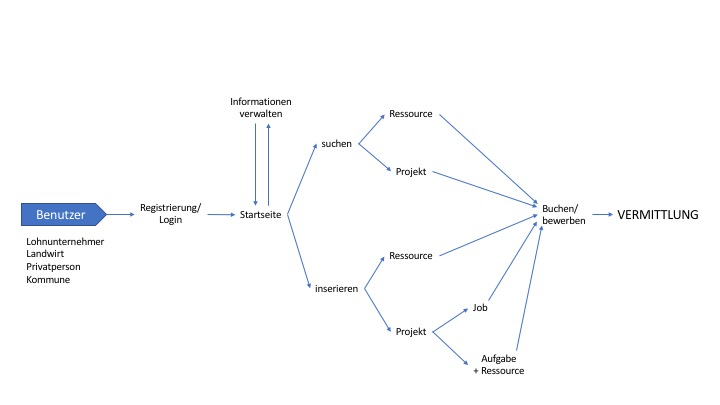
\includegraphics[width=\textwidth]{99_IMG/03_Umsetzung/map.jpg}
	\caption{Resultat der Sprint-Map von Agrishare}
	\label{fig:map}
\end{figure}
%
%Wie in \ref{fig:map} dargestellt ist, wurden die Benutzer nochmal in Einzelgruppen eingeteilt. Das diente dem besseren Verständis im Team. Diese Benutzer müssen sich zuerst authentifizieren durch Login oder Registrierung. Danach sollen sie auf die Startseite geleitet werden, von wo aus sie verschiedene Möglichkeiten haben sollen. Die Nutzer können dann ihre Informationen verwalten, nach Inseraten suchen oder selber inserieren. Bei der Suche wird nur zwischen Ressourcen oder Projekten unterschieden, wohingegen ein Inserat ebenfalls eine Ressource oder ein Projekt beinhalten kann, dieses aber nochmal in Job oder Aufgabe unterteilt ist. Eine Aufgabe ist so definiert, dass es auch Ressourcen beinhalten kann. Nach diesen Abläufen kommt es typischerweise zu einer Buchung oder Bewerbung. Nach der Bestätigung wurde also eine Vermittlung durchgeführt, was das Ende des Prozesses beschreibt.

\paragraph{Ask the Experts}
In Abschnitt \ref{sec:Sprint-Tag1-AtE} wird erläutert, dass diese Aufgabe dazu dienen soll, einzelne Teilbereiche des Projektes genauer zu erklären. Dafür werden Experten der einzelnen Themen eingeladen, um über diesen Bereich vorzutragen und Fragen dazu zu beantworten. 
Die Expertenrunden laufen in diesem Team zunächst wie geplant ab. Die meisten Fachleute kommen hier tatsächlich aus dem Sprint-Team selbst. So wird über die Bereiche Rechnungswesen und -stellung, typische Fehlerquellen und den aktuellen Vermittlungsvorgang vorgetragen. Diese Aufgabe ist grundlegend dafür gedacht, bereits Gehörtes erneut zu wiederholen und bei Unklarheiten Fragen zu stellen. So werden durch das Vortragen des letzten Experten, welcher ein potentieller Endkunde sein könnte, besonders viele neue Einblicke gewonnen. Als klarer Vertreter der Kundenseite, deutet dieser auf Unklarheiten bezüglich des Gesamtprojektes hin. Aufgrund der vielen wertvollen Informationen von diesem Experten wird das Gespräch nicht nach 30 Minuten abgebrochen, wie vorgegeben. Daher werden die restlichen geplanten Punkte für den ersten Tag auf Tag zwei verschoben. Das Projektteam ist sich bei dieser Prozessabwandlung einig, da das Gespräch mit diesem Experten jedem dabei hilft, den Kunden besser zu verstehen und das Projekt darauf zu beschränken, was der Kunde tatsächlich braucht.

Während aller Expertenrunden schreibt das restliche Team Notizen auf Klebezettel und legt diese beiseite. Am Ende werden alle Notizen gesammelt und an einem Whiteboard angebracht. Die geplanten weiteren Punkte werden, wie bereits erwähnt, auf Tag 2 verschoben.
%
%Experten:
%Theresa Jakob: Rechnungswesen
%Matthias Coufal, Verena Schmöller: Ablauf der Buchung über Maschinenring
%Sebastian Brunthaler: Typische Fehlerquellen in Projektteams
%Landwirt: allgemeiner Eindruck des Projektes, Unklarheiten?
%Masterand Horsch: Kundensicht
%
%Rechnungswesen: 
%Erhalten der Originalrechnung: Wenn per Post verschickt, Papierform ist Originalrechnung. Wenn per E-Mail verschickt, elektronische Form ist Originalrechnung (nicht der Ausdruck). 
%
%Fehlerquellen:
%Verschieben der Aufgaben von Person zu Person. Keine Verantwortung für eigene Aufgaben übernehmen.
%
%Prozess MR:
%Vermittlung der Maschinen/Dienstleistungen telefonisch. Meist nicht über MR, da sich Landwirte meist untereinander kennen. Abrechnung immer über MR, da der bürokratische Aufwand der Rechnungsstellung und Dieselbeihilfe abgenommen wird. Preis: Vorschläge von MR (Preiskatalog), aber individuell einstellbar.
%
%Kundensicht: Möglichkeit, Maschinen mit Versicherung zu vermieten. Lohnunternehmer-Prozess bisher, allerdings mehr Potential in Privatpersonen, da sehr große Zielgruppe. Fokus auf kleineren Hausarbeiten
%
%Da ein sehr hilfreicher potentieller Endkunde ebenfalls als Experte eingeladen wurde, welcher sehr viele Einsichten über potentielle Unklarheiten geben konnte, wurde der geplante Ablauf des Sprints bereits am Tag 1 abgewandelt. Es wurde der Fokus darauf gelegt, so viel wie möglich mit diesem Experten zu besprechen und die weiteren Punkte auf den nöchsten Tag zu legen.

\paragraph{Logo und Name}
Parallel zum eigentlichen Sprint-Prozess ist das Team an Tag 1 so motiviert, dass in den Pausen kleinere Diskussionen bezüglich Logo und Name des Produkts entstehen. Auf einem weiteren Whiteboard werden Skizzen und Begriffe gesammelt, welche innerhalb der Pausen, sowie vor und nach dem Workshop von allen Teilnehmern bewertet und abgeändert werden. Dabei ergeben sich wiederum Diskussionen und neue Ideen. Für die Teilnehmer bietet dies eine kreative Abwechslung zum eigentlichen Sprint-Programm. Das führt dazu, dass im Anschluss an den offiziellen Sprint das finale Logo und auch der letztendliche Produktname entstehen.

\paragraph{Fazit}
Nach dem ersten Tag ist das Gesamtfeedback des Teams durchaus positiv. Der Prozess wird bisher als hilfreich angesehen, obwohl die Erwartungen im Vorfeld verhältnismäßig niedrig waren. Unter Anderem war es möglich in nur einem Tag potentielle Risiken im Vorfeld zu eliminieren. Außerdem wird vermutet, dass die Entwicklung allgemein erleichtert wird, da Unklarheiten, welche sonst in der Implementierungszeit potentielle Probleme darstellen würden, bereits beseitigt sind. Da das ganze Team fokussiert und konzentriert mitarbeitet, ist der gesamte Tag äußerst produktiv. So entstehen auch viele Ideen bezüglich möglicher Erweiterungen und weiterer Anwendungsgebiete. Auch vorher verworfene Anwendungsgebiete werden wieder aufgerollt und ins Gedächtnis gerufen. Des Weiteren werden die Bedenken der Teilnehmer schriftlich festgehalten, was das Team durchaus positiv stimmt. Im Allgemeinen entstehen ertragreiche Diskussionen und Ideenfindungen. Es war auch wichtig, die Erwartungen aller Teammitglieder aufeinander abzustimmen und sicherzugehen, dass alle die gleichen Ansichten haben. Dabei geht es nicht nur um zeitliche Erwartungen, sondern auch was das Projekt beinhaltet und was tatsächlich das Produkt darstellen soll. Denn jedes Teammitglied hatte für sich selbst ein sehr klares Bild von dem Projekt. Diese Ansichten waren allerdings von Person zu Person sehr unterschiedlich, können jedoch angeglichen werden. Daher ist Tag 1 vor allem auch im Bereich 'Teambuilding' sehr erfolgreich.

Obwohl die Expertenrunden zunächst nicht sehr hilfreich scheinen, zeigt sich der Mehrwert davon dennoch. So sind die Notizen, welche während dieser Aufgabe entstehen, essentiell für den weiteren Verlauf des Projekts. Die Themen wurden zwar schon des Öfteren besprochen, jedoch nie schriftlich festgehalten. Daher ist es durchaus sinnvoll, diese Dinge aufzuschreiben, um zu garantieren, dass sie nicht in Vergessenheit geraten, wenn nicht mehr darüber diskutiert wird.

\subsection*{\refstepcounter{subsection}\label{sec:Sprint-Umsetzung-Tag2}\thesubsection\quad Tag 2}
\paragraph{Notizen sortieren und bewerten}
Da am Tag 1 nicht alle geplanten Aufgaben abgearbeitet werden können, müssen die letzten drei Punkte, welche in Abschnitt \ref{sec:Sprint-Tag1-Notizen} erklärt sind, am nächsten Tag behandelt werden. Diese nehmen allerdings nicht viel Zeit in Anspruch, sodass das Team schnell wieder in den eigentlichen Ablauf einsteigen kann. Das Sortieren und Bewerten der Notizen läuft ohne viele Diskussionen ab, da sich die Teilnehmer meist einig sind. So werden am Ende zwei Haftnotizen mit den meisten Stickern an der Map angebracht. 
%\paragraph{Fokus des Sprints}
Nun ist es die Aufgabe des Deciders, den Fokus für diesen Sprint einzugrenzen. Da das Projekt zu diesem Zeitpunkt noch am Anfang der Entwicklung steht, müssen für einen sinnvollen und testbaren Prototypen fast alle Bereiche der Map abgedeckt werden. Deshalb wird der Fokus auf die gesamte Map gerichtet, was in der Spezifikation nicht so vorgesehen ist. Jedoch hat der Decider entschieden, dass nur eine teilweise Prototypisierung des Projektes zu einseitige Ergebnisse hervorrufen würde und deshalb für das Endprodukt nicht hilfreich wäre.

%Zuerst werden die gesammelten Notizen sortiert. Dabei sortiert das gesamte Team zuerst Duplikate aus und teilt die restlichen Zettel in inhaltlich logische Gruppen ein. Für diese Gruppen wurden zusätzlich noch Überbegriffe festgelegt und ebenfalls an dem Whiteboard angebracht. Anschließend wurden Sticker verteilt - zwei Sticker pro Person und 4 für den Decider. Jedes Teammitglied sollte sich nun das Long Term Goal, sowie die Sprint-Fragen erneut vor Augen führen. Danach werden die Sticker in einer stillen Abstimmung an die Notizen angebracht, die für den Sprint-Zeitraum als am Wichtigsten erachtet werden. Diese Notizen wurden dann an dem Whiteboard mit der Map angebracht, passend zu den jeweiligen Schritten.


\paragraph{Lighting Demos}
%Liste mit für das Projekt interessante Produkte
%
%Liste:
%\begin{itemize}
%	\item Airbnb
%	\item Google Maps
%	\item Uber
%	\item Tractorpool
%	\item ...
%\end{itemize}
Die in Abschnitt \ref{sec:Sprint-Tag1-Demos} beschriebenen \textit{Lightning Demos} bezeichnen kurze Referate der Teammitglieder über etablierte Produkte mit Parallelen zu dem aktuellen Projekt. 
Hier beschäftigt sich jedes Teammitglied mit zwei bis drei Produkten und hebt für das Projekt relevante Teile hervor. Die Übung wird allgemein als eine gute Inspiration erachtet und es gibt nur wenige Diskussionen. 
Bei dieser Aufgabe fällt auf, dass zwar die meisten Produkte schon im Vorhinein bekannt waren, sich allerdings die Meinungen darüber im Team selbst sehr unterscheiden. Betrachtet werden unter Anderem Online-Dienste wie AirBnb, Uber und Ebay. AirBnb ist eine Plattform für die Vermietung von eigenem Wohnraum. Durch die Anwendung ist es möglich, das eigene Zimmer für einen kurzen Zeitraum zu vermieten, wobei sowohl Buchungsprozess, als auch der Bezahlvorgang von der Plattform abgewickelt werden. Hier wird besonders auf das Design, die Darstellung von Inseraten und den Buchungsvorgang eingegangen. Dagegen stellt Uber eine Plattform für die Vermittlung von Personenbeförderungsdienstleistungen dar. Hier kann eine Person durch die Angabe von Start- und Zielposition einen geeigneten Fahrer finden, buchen und bezahlen. Diese Anwendung hebt sich vor allem durch die schnelle und einfache Benutzung hervor, was für Agrishare auch von großer Bedeutung ist.

Die anschließende Aufgabenverteilung erfolgt reibungslos, da sich das Team schnell darauf einigen kann, wer welche Bereiche bearbeiten soll. Da der Fokus in diesem Fall breit gefächert ist, werden jeder Person jeweils 3 Schritte zugeteilt.

\paragraph{Sketch}
\label{ref:Sprint-Umsetzung-Sketch}
Der Prozess des \textit{Sketching} ist nach Eric Ries in mehrere Schritte aufgeteilt, welche in Abschnitt \ref{sec:Sprint-Tag2-Sketch} beschrieben sind. Nach dieser Vorgabe beginnt das Team, Notizen und erste Ideen stichpunktartig zusammenzutragen. Bereits nach den ersten 30 Minuten der Ideensammlung fällt auf, dass der Prozess so nicht hilfreich für das Projekt ist. Es werden zu viele Screens für den Prototypen benötigt, welche unmöglich innerhalb der kurzen Zeit von wenigen Personen erstellt werden können. Außerdem ist es besonders wichtig, dass die Screens eine einheitliche Maske und einen ähnlichen Aufbau haben. Deshalb ist es nicht sinnvoll, jede Person ein eigenes Set an Bildschirmen bauen zu lassen. Nachdem also jeder eigene Ideen gesammelt hat, wird begonnen, die einzelnen Seiten mit der gesamten Gruppe groß auf einem Whiteboard zu erstellen. Hier fällt auf, dass es immer noch einige Unklarheiten bezüglich der grundlegenden Funktionsweise gibt. Das Team führt sich allerdings immer wieder vor Augen, dass das Endprodukt nicht besonders kreativ gestaltet, sondern einfach zu verstehen und nach einem einheitlichen Prinzip aufgebaut sein muss. Innerhalb des Nachmittags von Tag 2 schafft es das Team, eine einheitliche Maske zu erstellen und es kann die Startseite, sowie teilweise die Kartenansicht erstellt werden.
Zugunsten des Projekterfolges wird am Ende von Tag 2 beschlossen, die Screens nach einem eigenen Prozess in Gruppenarbeit zu erstellen, anstatt dem Sprint-Prozess zu folgen.

\paragraph{Fazit}
Am Ende von Tag 2 ist das Team wiederum einer Meinung, was den Gesamtprozess angeht. Der Sketch-Prozess, wie spezifiziert, ist nicht sinnvoll für ein einheitliches Produkt mit vielen Screens. Das heißt nicht, dass die Herangehensweise grundsätzlich als falsch angesehen wird. Für kleinere Add-Ons, funktionelle Erweiterungen oder Design-Fragen könnte dies durchaus einen großen Mehrwert gegenüber der abgeänderten Herangehensweise haben. Nichtsdestotrotz war das Projektteam kreativ und aufmerksam.  Auch die Befürchtung, man könnte sich an unnötigen Details aufhängen, kann nicht bestätigt weden, da dies immer sehr gut eliminiert werden konnte. Da zu diesem Zeitpunkt bereits der komplette Sprint-Prozess abgewandelt wurde, sind die Rollen zwangsläufig ineinander verschmolzen.

\subsection*{\refstepcounter{subsection}\label{sec:Sprint-Umsetzung-Tag3}\thesubsection\quad Tag 3}Der Tag wird so begonnen, wie der Tag zuvor beendet wurde, mit dem Erstellen der verschiedenen Screens des Endproduktes mit dem gesamten Team. Um Zeit einzusparen, erstellt ein Teammitglied parallel dazu den digitalen Prototypen der erstellten Bildschirme. Obwohl der Tag wenig abwechslungsreich ist und eintönig scheint, ist das Team dennoch fokussiert und produktiv. Es entstehen wiederum zahlreiche Diskussionen, wobei man sich aber auf essentielle Dinge beschränkt. Beispielsweise wird die Kartenansicht, welche in Abbildung \ref{fig:mapWireframe} dargestellt ist, fertiggestellt. In dieser Abbildung ist auch die Maske, welche am Tag zuvor erstelle wurde, klar zu erkennen. Diese besteht aus einer Seitenleiste mit unterschiedlichen Reitern. Das Team eintscheidet sich für eine Leiste, um dem Kunden eine einfache Benutzung der Plattform zu ermöglichen, indem alle Funktionen zu jeder Zeit deutlich sichtbar sind. Dieses Konzept lässt sich auf allen im Sprint entwickelten Oberflächen wiederfinden. In späteren Nutzertests stellt sich die Seitenleiste jedoch als verwirrend heraus. Verschiedene Testpersonen beschreiben diese unter Anderem als zu kompliziert aufgebaut und unnötig. Daher werden die in die Leiste eingebauten Reiter komprimiert und in einen Header eingebaut, welcher in der implementierten Version der Karte auf Abb. \ref{fig:mapScreenshot} dargestellt ist. Diese Änderung wird im Rahmen erneuter Nutzer-Tests positiv bewertet. Damit ist es möglich, die Karte über die gesamte Breite der Ansicht zu strecken, was ebenfalls von den Kunden als gut empfunden wird.  

\begin{figure}
    \centering
    \begin{subfigure}[b]{0.45\textwidth}
        \includegraphics[width=\textwidth]{99_IMG/03_Umsetzung/mapWireframe_3.jpg}
        \caption{Skizze der Kartenansicht}
        \label{fig:mapWireframe}
    \end{subfigure}
    ~ %add desired spacing between images, e. g. ~, \quad, \qquad, \hfill etc. 
      %(or a blank line to force the subfigure onto a new line)
    \begin{subfigure}[b]{0.45\textwidth}
        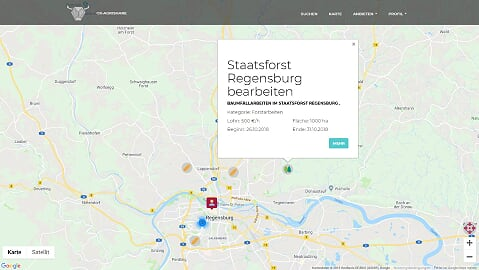
\includegraphics[width=\textwidth]{99_IMG/03_Umsetzung/mapScreenshot.jpg}
        \caption{Screenshot der Kartenansicht}
        \label{fig:mapScreenshot}
    \end{subfigure}
    \caption{Gegenüberstellung von Skizze und Implementierung der Kartenansicht der Plattform Agrishare}\label{fig:mapView}
\end{figure}

\subsection*{\refstepcounter{subsection}\label{sec:Sprint-Umsetzung-Tag4}\thesubsection\quad Tag 4}Bereits zu Beginn von Tag 4 wird klar, dass es wenig Sinn macht, den Prototypen so zu testen, da dieser noch zu wenig Inhalt hat. Deshalb wird beschlossen, die geplanten Tests zu verschieben und direkt nach dem Sprint damit zu beginnen, das Produkt ansatzweise zu implementieren. Ein weiterer Grund dafür, die Tests abzusagen, ist, dass ein Usertest mit unserer Zielgruppe zu viel Aufwand für einen Tag wäre. Denn Landwirte sind vor allem im Sommer sehr beschäftigt und können nicht für 30 Minuten in die Stadt fahren. Deshalb wird beschlossen, zu einem späteren Zeitpunkt potentielle Tester zu besuchen und dort zu testen. Das Team führt die Erstellung der einzelnen Bildschirme fort, wie bereits an Tag 3. An diesem Tag wird hauptsächlich an der Startseite gearbeitet. Da dieser Screen einen Blickfang für potentielle Neukunden darstellen soll, gibt es einige Diskussionen über den grundlegenden Aufbau. Hier wird bereits das Konzept einer Kopfzeile umgesetzt, da eine Seitenleiste auf dieser Ansicht als überflüssig angesehen wird. In den anschließenden Tests sorgt dies für zusätzliches negatives Feedback. Die Skizze der Startseite, sowie die Implementierung sind in Abb. \ref{fig:homeView} dargestellt.

\begin{figure}
    \centering
    \begin{subfigure}[b]{0.45\textwidth}
		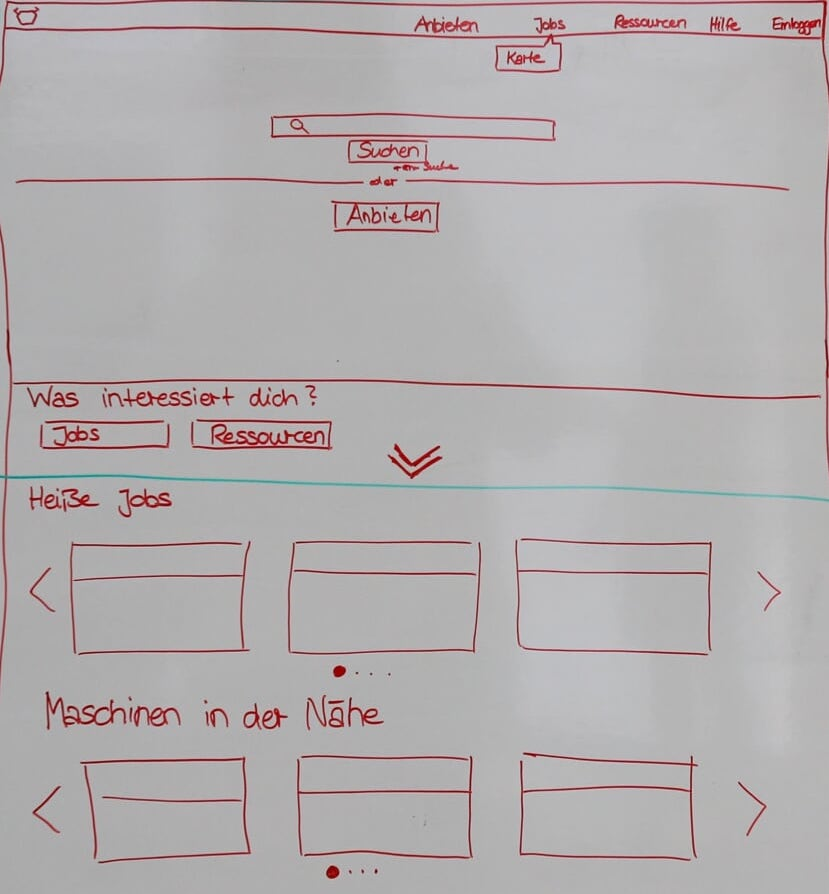
\includegraphics[width=\textwidth]{99_IMG/03_Umsetzung/homeWireframe_5.jpg}
		\caption{Skizze des Startbildschirmes}
		\label{fig:homeWireframe}
    \end{subfigure}
    ~ %add desired spacing between images, e. g. ~, \quad, \qquad, \hfill etc. 
      %(or a blank line to force the subfigure onto a new line)
    \begin{subfigure}[b]{0.45\textwidth}
        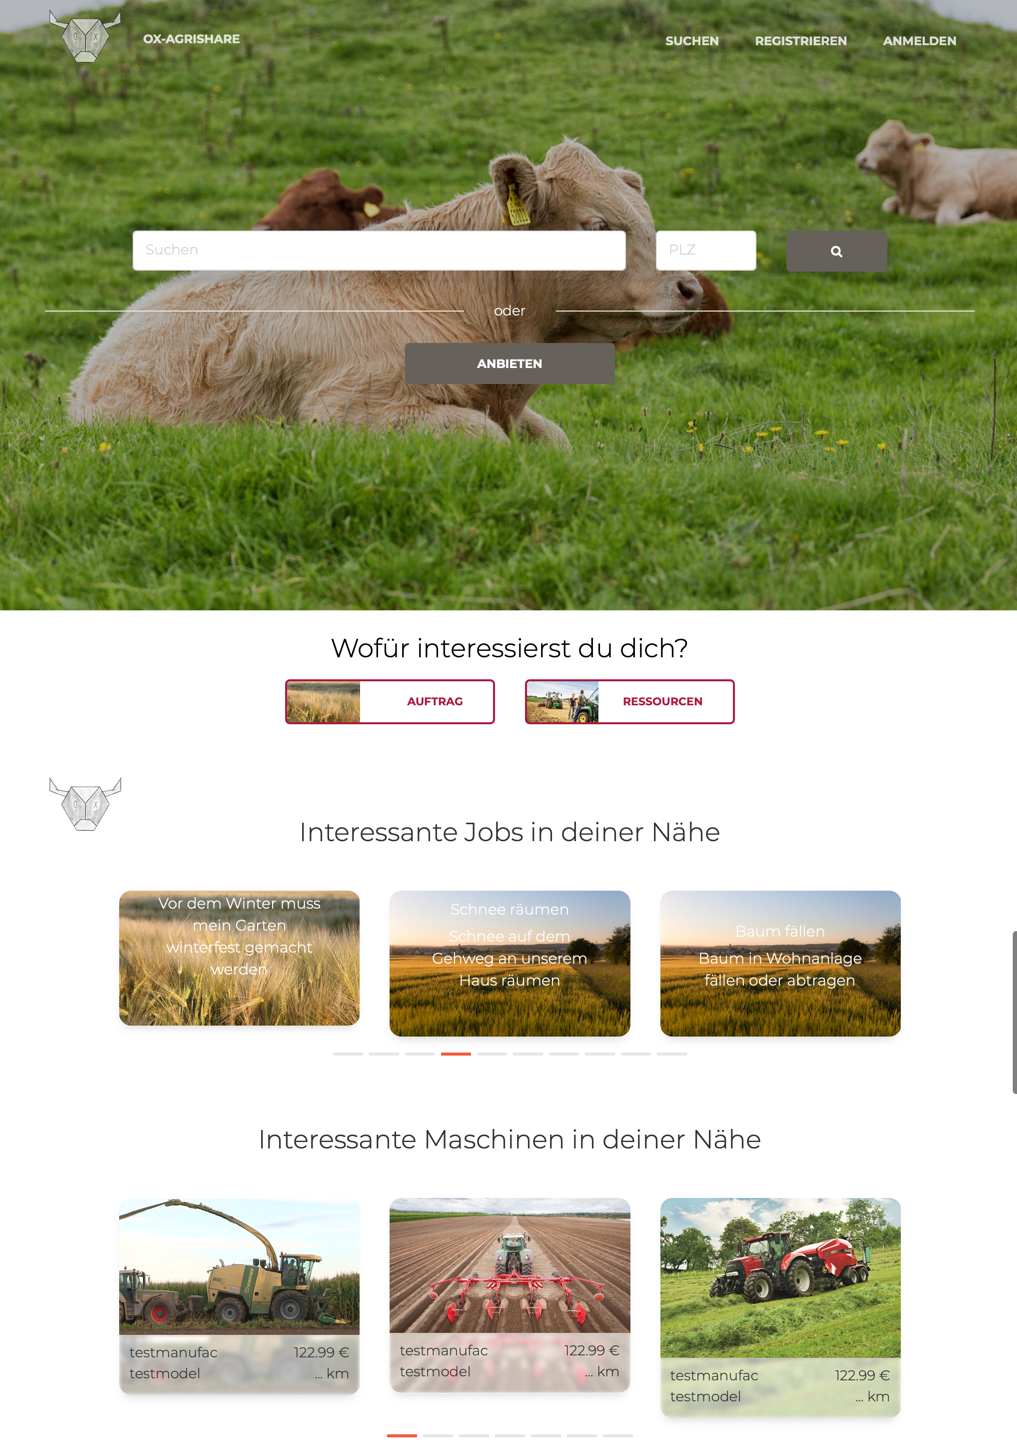
\includegraphics[width=\textwidth]{99_IMG/03_Umsetzung/homeScreenshot.png}
        \caption{Screenshot des Startbildschirmes}
        \label{fig:mapScreenshot}
    \end{subfigure}
    \caption{Gegenüberstellung von Skizze und Implementierung der Hauptseite der Plattform Agrishare}\label{fig:homeView}
\end{figure}

\subsection*{\refstepcounter{subsection}\label{sec:Sprint-Umsetzung-Tag5}\thesubsection\quad Tag 5}Am letzten Tag sind fast alle Screens fertig skizziert. Die wird restliche Zeit wird genutzt, um nochmal alle Details zu klären, die restlichen Screens zu erstellen und sich auf ein Logo und einen Namen zu einigen. Dieses Ziel wird erreicht und das Team schließt den Sprint mit einem sehr guten Gefühl ab. Das finale Logo ist in Abb. \ref{fig:logoAgrishare} dargestellt. Durch unterschiedliche Kombinationen mehrerer Skizzen und Ideen entsteht dieses Logo über den gesamten Zeitraum des Workshops. Aus dieser Darstellung entwickelt sich ebenfalls der Name der Plattform \textit{OX}. Dieser wird jedoch nach dem Sprint verworfen und das Team beschließt den Namen \textit{Agrishare} beizubehalten. 
\begin{wrapfigure}{r}{0.5\textwidth}
%\vspace{-20pt}
	\begin{center}
		
\includegraphics[width=0.48\textwidth]{99_IMG/03_Umsetzung/Skizzeheller.png}
	\end{center}
	\vspace{-20pt}
  \caption{Im Sprint erstelltest Logo des Startups Agrishare}
		\label{fig:logoAgrishare}
  \vspace{-40pt}
\end{wrapfigure}

%\subsection*{Allgemeines Fazit - Sprint}

\subsection*{Evaluierung des Prozesses}
Wie bereits angedeutet, hatte das Projektteam keine klare Vorstellung davon, welche Erwartungen es an den Prozess des Sprints stellen sollte. Am Ende war das Team jedoch positiv über die Erkenntnisse aus dem Event überrascht. Hauptsächlich die ersten beiden Tage haben dem Team vermutlich viel Arbeit und zukünftige Diskussionen erspart. Positiv anzumerken ist, dass jeder Beteiligte aufmerksam mitgearbeitet hat und mit großem Arbeitswillen bei der Sache war. Das führte dazu, dass das Team während der ganzen 5 Tage hochkonzentriert war und dementsprechend sehr gute Arbeit und konstruktive Beiträge geleistet hat. Allerdings ist auch aufgefallen, dass der Prozess, wie vorgesehen, nicht sinnvoll für die Erstellung des komplett neuen Produktes Agrishare ist. Dies beinhaltet zu viele Einzelteile und zu viele Details, die das ganze Team zusammen abklären muss. Durchaus sinnvoll wäre das für eine Erweiterung eines bestehenden Produktes. In der abgewandelten Variante dieses Teams wurden trotzdem viel mehr Ergebnisse erzielt als erwartet. In nur fünf Tagen konnte ein Konzept erstellt werden, alle Screens des Produktes gezeichnet werden und sich auf ein Logo und einen Brand-Name geeinigt werden. Da alle Teammitglieder hauptberuflich andere Dinge machen, wie ein Studium oder Vollzeitarbeit, hätte es ohne den Sprint wohl sehr lange gedauert, bis diese Dinge geklärt worden wären.

Diesbezüglich war sich das Team auch einig, einen weiteren, auf diese Ergebnisse aufbauenden Sprint zu starten, sobald das Grundprodukt implementiert ist und erste User-Tests gemacht wurden.

\section{The Lean Startup}
\label{sec:LeanStartup}
\ac{TLS} beschreibt eine Sammlung an Konzepten, welche sich, nach \citeA{TheLeanStartup}, bei der Gründung von Startups als erfolgreich erwiesen haben. Der \ac{TLS}-Ansatz besteht aus unterschiedlichen Methoden, welche häufigen Fehlern im Umgang mit Startups entgegenwirken sollen, um diese Firmen vor dem Scheitern zu bewahren.

Der Autor grenzt ein Startup mit einer eigenen Definition der Unternehmensform klar von etablierten Firmen ab:
\begin{quote}
,,A human institution designed to create new products and services under conditions of extreme uncertainty.'' \cite[S. 8]{TheLeanStartup}
\end{quote}
Das Schlüsselwort \textit{uncertainty} - zu deutsch: Unsicherheit - in diesem Satz ist essentiell, da eine große Herausforderung eines Startups darin besteht, ein Produkt zu entwickeln, welches den Endnutzern einen Vorteil bietet. Im Gegensatz zu etablierten Unternehmen, welche bereits viele Erfahrungen mit dem Verhalten der Kunden haben, sind die Wünsche und Bedürfnisse der Kunden für ein Startup vorerst unbekannt. Daher entstehen Vermutungen über das Verhalten der Zielgruppe, welche meist nicht belegt werden können. Durch unbeweisbare Annahmen ensteht diese Unsicherheit. Deshalb ist das Hauptziel des \ac{TLS}-Modells, diese zu minimieren indem sämtliche Hypothesen über die Wünsche und Bedürfnisse der potentiellen Kunden im Rahmen von Tests geprüft werden. Dadurch können sichere Rückschlüsse gezogen werden, was wiederum das Gesamtrisiko minimiert.

Die genannten Konzepte werden im Folgenden genauer erläutert.

\subsection*{\refstepcounter{subsection}\label{sec:LeanStartup-ValidatedLearning}\thesubsection\quad Validated Learning}
Bei Startups entsteht oft das Problem, dass Erfolg zu Beginn nicht nach traditionellen Methoden gemessen werden kann. In einem etablierten Unternehmen gibt es für ein Projekt exakte Zeit- und Budgetvorgaben, welche einzuhalten sind. Ist dies gelungen, gilt das Projekt als erfolgreich. Wendet man diese Methode bei einem Startup an, ist es möglich, dass diese Vorgaben zwar eingehalten werden, jedoch wird das Produkt nicht verkauft, da es keine Nachfrage dafür gibt. In diesem Fall war das Projekt nach klassischem Denken erfolgreich, das Produkt allerdings nicht. Nach der gesamten Projektlaufzeit hat das Unternehmen dabei gelernt, dass das Produkt geändert werden muss. \citeauthor{TheLeanStartup} erklärt, dass dieses Wissen bereits in einer kürzeren Zeitspanne erlangt werden kann. Dafür entwickelt er eine Herangehensweise, welche \ac{VL} genannt wird. Diese wurde entwickelt, um Fortschritt im Sinne von Wissen über die Zielgruppe nachzuweisen und zu demonstrieren. Im Gegensatz zu klassischen Prognosen über den Markt und Produkterfolg werden mit Hilfe von \ac{VL} im Rahmen von empirischen Beobachtungen nachweisbare Ergebnisse erbracht. Das Grundprinzip besteht darin, grundsätzliche Annahmen über den Endnutzer und das Produkt in kleineren Experimenten zu testen. Das heißt, sämtliche Vermutungen über die Wünsche oder Bedürfnisse der Zielgruppe werden im Rahmen der \ac{BML} Schleife, welche in Abschnitt \ref{sec:LeanStartup-BML} genauer erklärt wird, geprüft. Damit kann die Richtigkeit dieser Annahmen im Vorfeld gesichert werden. So können bereits im frühen Stadium der Entwicklung viele Risiken eliminiert werden, da das Verhalten der Nutzer von Anfang an getestet anstatt abgeschätzt wird.

Durch diese empirischen Daten kann ein Startup viele messbare Einblicke über die Zielgruppe hervorbringen. Je genauer die Wünsche und Bedürfnisse der Endkunden bekannt sind, desto einfacher ist es im Umkehrschluss, ein auf die Nutzer abgestimmtes Produkt zu entwickeln. Daher stellt jeder Einblick eine eigene Einheit für Fortschritt dar, erklärt \citeauthor{TheLeanStartup}.

\subsection*{\refstepcounter{subsection}\label{sec:LeanStartup-BML}\thesubsection\quad Bauen-Messen-Lernen}
\begin{figure}
	\begin{center}
		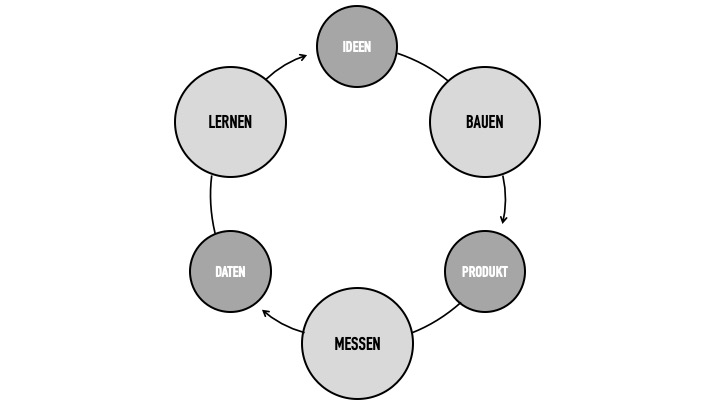
\includegraphics[scale=0.5]{99_IMG/02_Grundlagen/buildmeasurelearn.jpg}
		\caption[Modell der \ac{BML} Schleife nach dem \ac{TLS}-Konzept.]{Modell der \ac{BML} Schleife nach dem \ac{TLS}-Konzept (Abbildung übersetzt aus \citeNP{TheLeanStartup}).}
		\label{fig:LeanStartup_BuildMeasureLearn}
	\end{center}
\end{figure}
Wie in Abb. \ref{fig:LeanStartup_BuildMeasureLearn} dargestellt, beschreibt dies eine Abfolge von Aufgaben, die maximalen Lerneffekt versprechen. Diese wird oft wiederholt, um neue Einsichten zu gewinnen. Daher entsteht pro Iteration ein neuer Lerneffekt, da bei jedem Durchlauf ein anderer Baustein getestet wird. Um diese Details zu definieren, wird die Schleife rückwärts geplant. Erst muss festgelegt werden, welche Einblicke in dieser Iteration wichtig sind bzw. was genau im Rahmen dieser Iteration herausgefunden werden soll. Mit dieser Grundlage wird dann beschlossen, welche Messungen nötig sind, um die richtigen und eindeutigen Einblicke zu bekommen. Danach kann erst entschieden werden, was dafür gebaut werden muss. Dabei kann es sich um einzelne Zusatzfunktionen handeln, aber auch um ein komplettes Produkt. Bei einem neuen Produkt ist es wichtig, nur die Schlüsselfunktionen zu entwickeln, also den Kern des Endproduktes. Darunter versteht man auch ein \textit{\ac{MVP}}. Das ist eine Version des Produktes, welche einen kompletten Durchlauf der Schleife bei minimaler Entwicklungszeit ermöglicht. Dabei ist es plausibel, dass unnötige Details weggelassen werden müssen, da diese den Aufwand erhöhen würden, ohne einen Mehrwert nach sich zu ziehen.

\subsection*{\refstepcounter{subsection}\label{sec:LeanStartup-InnovationAccounting}\thesubsection\quad Innovation Accounting}
Die \textit{Innovation Accounting}-Methode ermöglicht es Startups, anhand von objektiven Beobachtungen und messbaren Erfolgen ein erfolgreiches Unternehmen aufzubauen, so \citeauthor{TheLeanStartup}. Zuerst wird ein \ac{MVP} entwickelt und getestet, um den Ausgangszustand des Startups einzuschätzen. Davon ausgehend wird die \ac{BML}-Schleife so oft durchlaufen, bis alle Annahmen über den Nutzer getestet und validiert sind. Schritt für Schritt entwickelt sich hier das Anfangsprodukt zu dem auf die Zielgruppe zugeschnittenen idealen Produkt. Solange das Unternehmen Fortschritte macht, gute Einblicke in die Kundensicht erhält und diese effektiv umsetzt, bewegt sich das Unternehmen weiter in Richtung Ideal. Ist das nicht der Fall, ist es unter Umständen Zeit für ein \textit{Pivot}, eine Methode, welche in Abschnitt \ref{sec:LeanStartup-Pivot} behandelt wird.

\subsection*{\refstepcounter{subsection}\label{sec:LeanStartup-Pivot}\thesubsection\quad Pivot}
\begin{figure}
	\begin{center}
		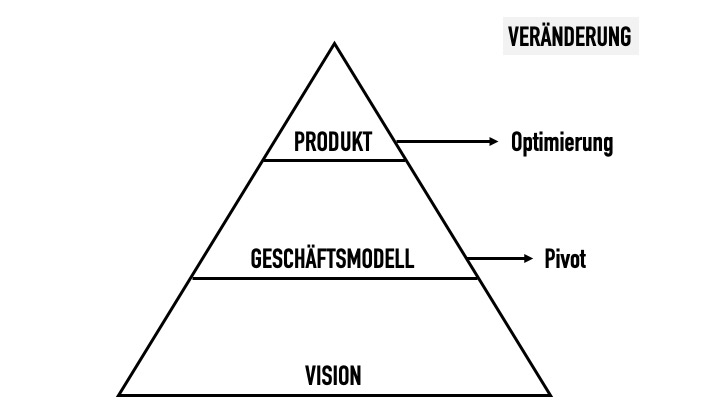
\includegraphics[scale=0.5]{99_IMG/02_Grundlagen/visionStrategyProduct.jpg}
		\caption[Unterteilung eines Projektes im \ac{TLS}-Modell.]{Unterteilung eines Projektes im \ac{TLS}-Modell (Abbildung übersetzt aus \citeNP{TheLeanStartup}).}
		\label{fig:LeanStartup_VisionStrategyProduct}
	\end{center}
\end{figure}
Unter einem \textit{Pivot} versteht man im Allgemeinen eine Kurskorrektur oder Abänderung des Geschäftsmodells. Nach \citeauthor{TheLeanStartup} ist jedes Startup-Projekt in drei Bausteine aufgeteilt. Diese werden Vision, Geschäftsmodell und Produkt genannt. Der Aufbau dieser Teile ist in der Abbildung \ref{fig:LeanStartup_VisionStrategyProduct} dargestellt. 
Die Vision liegt jeder Idee zugrunde. Sie beschreibt das Ziel, welches durch das Projekt auf lange Sicht erreicht werden soll. Die Vision selbst wird selten geändert, da sie der Grundbaustein des gesamten Startups ist. Darauf aufbauend entwickelt sich ein Geschäftsmodell nach dem das Produkt im Wesentlichen entwickelt wird. Die wichtigste und zugleich schwierigste Aufgabe eines Gründers ist zu entscheiden, wann sich das Geschäftsmodell des Projektes ändern muss. Der Autor empfiehlt dafür am Ende jeder \ac{BML}-Iteration ein \textit{Pivot}-Meeting einzuberufen. In diesem wird besprochen, ob das Experiment erfolgreich war oder nicht. Falls nicht, muss entschieden werden, ob das negative Ergebnis dem Geschäftsmodell geschuldet ist oder dem Produkt. Wie in Abb. \ref{fig:LeanStartup_VisionStrategyProduct} dargestellt, liegt der Unterschied darin, dass entweder ein \textit{Pivot} oder eine Feinabstimmung stattfinden muss. Dafür stellt \citeauthor{TheLeanStartup} unterschiedliche \textit{Pivot}-Modelle dar:
\begin{itemize}
	\item \textbf{Zoom-in Pivot:} Das neue Produkt besteht aus einem einzelnen Baustein des ursprünglich geplanten Produktes.
	\item \textbf{Zoom-out Pivot:} Das neue Produkt enthält das ursprünglich geplante Produkt als Feature.
	\item \textbf{Customer Segment Pivot:} Das Produkt wird auf eine andere Zielgruppe, als ursprünglich geplant, zugeschnitten.
	\item \textbf{Customer Need Pivot:} Das Produkt wird dahingehend abgeändert, dass ein unterschiedliches Problem der gleichen Zielgruppe damit gelöst wird. Das heißt, es stellt sich heraus, dass die Nutzer, mit denen zusammengearbeitet wird, andere Bedürfnisse haben, als ursprünglich angenommen.
	\item \textbf{Platform Pivot:} Software, welche ursprünglich als App geplant wurde, wird als Plattform realisiert oder umgekehrt.
	\item \textbf{Business Architecture Pivot:} Dieser Pivot beinhaltet den Wechsel vom B2B zum B2C Geschäft und umgekehrt.
	\item \textbf{Value Capture Pivot:} Die Art, durch welche das Produkt einen Wert für den Kunden erzeugt, wird geändert. 
	\item \textbf{Engine of Growth Pivot:} Der Erfolg des Produktes wird durch eine andere Methode gemessen. Die unterschiedlichen \textit{Engines of Growth} werden in Kapitel \ref{sec:LeanStartup-EnginesOfGrowth} erklärt.
	\item \textbf{Channel Pivot:} Der Vetriebskanal wird geändert. So wird das Produkt auf einem anderen Weg, als ursprünglich geplant, an den Kunden gebracht.
	\item \textbf{Technology Pivot:} Das Produkt wird auf technischer Ebene abgeändert. Das soll bessere Preisangebote oder Performance mit sich ziehen.
\end{itemize}
Ein Geschäftsmodell während der Entwicklung abzuändern, stellt eine große Schwierigkeit dar. Da es keine optimale Strategie für die Produktentwicklung gibt, muss jedes Startup ein eigenes Modell entwickeln, um maximalen Erfolg zu erzielen. Daher ist die Entschiedung, ein \textit{Pivot} durchzuführen, subjektiv und nicht messbar. Außerdem gibt es keine Garantie für den Erfolg des neuen oder abgeänderten Konzeptes. 

Das Geschäftsmodell ist wiederum das Fundament für das Endprodukt. Dies soll nach jeder Iteration abgewandelt werden, um den Wünschen und Bedürfnissen der Endkunden gerecht zu werden. Diese Änderungen werden demnach als Optimierung bezeichnet, da es sich um kleinere Anpassungen des Produktes handelt. Eine große Herausforderung für ein Startup ist es, diese drei Bausteine so anzupassen, dass ein erfolgreiches Unternehmen daraus entstehen kann.

\subsection*{\refstepcounter{subsection}\label{sec:LeanStartup-Batches}\thesubsection\quad Batches}
Etablierte Unternehmen fertigen Produkte meist in großen Mengen an. Dafür sind verschiedene Abteilungen für unterschiedliche Teile des Endproduktes verantwortlich. Oft werden erst Vielzahlen der Einzelteile produziert, bevor sie weitergegeben werden. Die Probleme, die \citeauthor{TheLeanStartup} dabei auffallen, sind unter Anderem, dass Fehler in den Teilen erst spät erkannt werden und dann die gesamte Charge neu gefertigt werden muss. Dasselbe gilt für Inkompatibilität. Falls ein Einzelteil aufgrund unzureichender Planung falsch entworfen wurde, fällt das erst spät im Fertigungsprozess auf. Daher empfiehlt der Autor für Startups kleinere Mengen des Produktes herzustellen, da es hier öfter dazu kommen kann, dass das Produkt nicht fehlerlos durchgeplant ist. Die Einzelteile werden hier sofort an die nächste Instanz weitergegeben um Unstimmigkeiten zeitnah abzuklären. Außerdem verringert dies die Fertigungszeit für die ersten Produkte, welche schneller an den Kunden gebracht werden können, um konstruktives Feedback einzuholen. Die schnelle Fertigung ist wiederum mit der \ac{BML} Schleife vereinbar.

\subsection*{\refstepcounter{subsection}\label{sec:LeanStartup-EnginesOfGrowth}\thesubsection\quad Erfolge messen - Engines of Growth}
Nach \citeauthor{TheLeanStartup} gibt es drei Konzepte, nach welchen Wachstum in einem Startup gemessen werden kann. Auch hier beruft er sich auf die Unsicherheit über die Zielgruppe, die ein Startup grundlegend von einem etablierten Unternehmen unterscheidet. Zweitere können das Unternehmenswachstum meist an Umsatzquoten erheben, was für neue Firmen oft nicht aussagekräftig ist. Daher ist es sinnvoll, hier eine andere Metrik zu benutzen. Er bezeichnet diese Konzepte als die \textit{sticky}, \textit{viral} und \textit{paid} Wachstumsmotoren, welche im Folgenden genauer erläutert werden.

\begin{itemize}
	\item \textbf{Sticky engine of growth}
	
	Bei dieser Methode liegt der Fokus auf zwei Gruppen von Nutzern. Die Kunden, die aufhören, das Produkt zu benutzen, genannt \textit{Churn Rate}, und neu gewonnene Nutzer, welche die \textit{Neukundenrate} bilden. Übersteigt die \textit{Neukundenrate} die \textit{Churn Rate}, wächst das Unternehmen. Daher liegt der Schwerpunkt hier darauf, die Nutzer an das Produkt zu binden, sodass die \textit{Churn Rate} niedrig gehalten wird. Dazu soll die \textit{Neukundenrate} möglichst hoch gehalten werden, was durch Marketing erreicht wird. So ist diese Methode besonders sinnvoll für Startups, die ihre Kunden langfristig an das Unternehmen binden wollen.
	\item \textbf{Viral engine of growth}
	
	Hier wird der sogenannte \textit{Viralkoeffizient} gemessen. Je höher dieser ist, desto schneller wächst das Startup. Berechnet wird dieser Koeffizient als Angabe der Neukunden, die pro Bestandskunde angeworben werden. Das heißt, falls jeder Bestandskunde im Durchschnitt einen Neukunden anwirbt, welcher wiederum einen Neukunden anwirbt etc, beträgt der \textit{Viralkoeffizient} gleich 1. Daraus ergibt sich exponentielles Wachstum, falls dieser Wert größer als 1 ist.
	\item \textbf{Paid engine of growth}
	
	Diese Methode stellt die Einnahmen pro Neukunde den Ausgaben dafür gegenüber. Das heißt, Marketingausgaben pro gewonnenem Kunden müssen geringer gehalten werden, als der \textit{Lifetime Wert} dieses Nutzers. Dieser beschreibt den Gesamtumsatz, den ein Unternehmen während seiner gesamten Nutzungszeit mit einem Kunden macht.
\end{itemize}

Es ist durchaus möglich, mehr als ein Konzept anzuwenden. \citeauthor{TheLeanStartup} empfiehlt allerdings, sich für eine Methode zu entscheiden. Der Grund dafür ist das hohe Verwirrungsrisiko. Daher ist es einheitlicher und einfacher zu verstehen, eine Methode zu verwenden. Welche der drei Konzepte am besten geeignet ist, ist abhängig von dem Endprodukt. Lebt das Produkt beispielsweise davon, eine Community mit vielen Nutzern zu haben, stellt sich der \textit{viral engine of growth} als sinnvoll dar. Da der Fokus hier darauf liegt, maximale Nutzerzahlen durch Mundpropaganda zu erreichen, ist dies hier eine optimale Methode, Wachstum zu messen.
\cite{TheLeanStartup}
\section{Business Model Canvas}
Durch die Erkenntnisse der vorherigen Konzepte erstellt das Agrishare-Team ein \ac{BMC}, welches in Abschnitt \ref{BMC_Kapitel} genauer erklärt wird. Ein erster Entwurf der Canvas ist in Abb. \ref{BMC_Agrishare} dargestellt.
\begin{figure}[h!]
		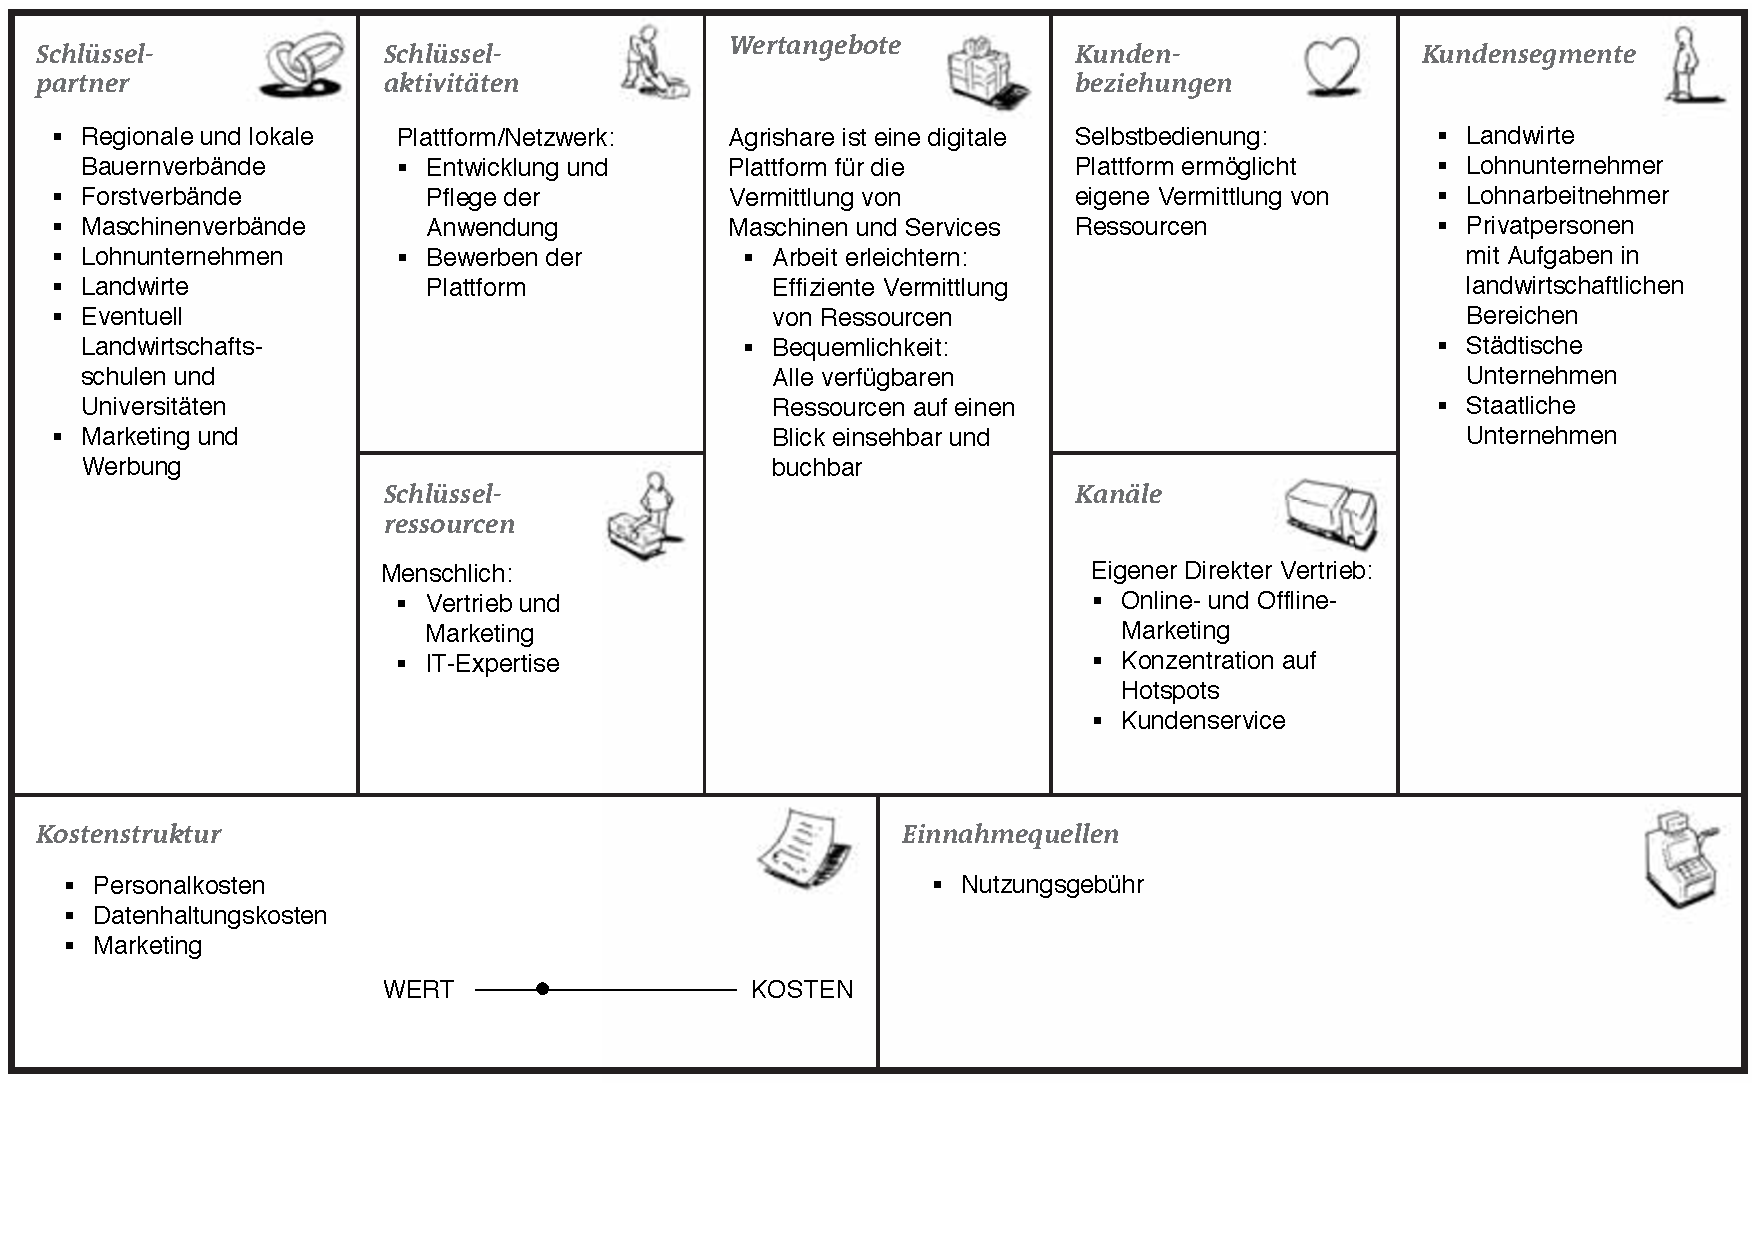
\includegraphics[angle=90,origin=c,width=\textwidth]{99_PDF_INCLUDE/BMC_draft.pdf}
		\caption{\ac{BMC} Agrishare}
		\label{BMC_Agrishare}
\end{figure}

Das Kundensegment ist hier als Nischenmarkt anzusehen, da es vorerst ausschließlich für die Landwirtschaft gedacht ist. Dieser Nischenmarkt kann zusätzlich in einzelne Segmente unterteilt werden, wie Landwirte, Lohnunternehmer und Lohnarbeiter, sowie Privatpersonen mit Aufgaben in landwirtschaftlichen Bereichen. Diese Nutzergruppen haben zwar ähnliche Bedürfnisse im Bezug auf die Agrarbranche, weisen aber unterschiedliche Eigenschaften auf. So bieten Lohnunternehmer und -arbeiter beispielsweise eine Dienstleistung an, die einem Landwirt zu Gute kommen kann. Das heißt, die selektive Kundengruppe der Lohnarbeiter kann ein Problem der Landwirte lösen, indem offene Tätigkeiten verrichtet werden. Im Umkehrschluss stellt ein Landwirt dem Lohnarbeiter bezahlte Tätigkeiten zur Verfügung, was wiederum ein Bedürfnis des Lohnunternehmers befriedigt. Das Ziel ist also, durch die Vernetzung dieser Kundensegmente einen Wert zu schaffen, von dem alle Nutzergruppen profitieren. Außerdem werden Städtische und Staatliche Unternehmen als weiteres Kundensegment angesehen, da diese ebenfalls Aufträge vergeben, welche sie nicht selber verrichten können. Damit können sie, ähnlich zu Landwirten, als Auftraggeber einen Nutzen aus der Plattform ziehen.

Die fundamentalen Werte, die Agrishare den Endkunden vermittelt, sind eine Arbeitserleichterung und Bequemlichkeit. In der Agrarbranche findet diese Vermittlung von Ressourcen bereits statt, jedoch nicht digital. Das bedeutet, dass die Plattform einen existierenden Prozess schneller, leichter und bequemer macht, indem die Nutzer benötigte Ressourcen online buchen können. Das erspart dem Kunden Arbeitsaufwand, da alle verfügbaren Maschinen und Dienstleistungen, sowie Aufträge auf einen Blick ersichtlich und sofort buchbar sind. Im Gegensatz dazu muss sich ein Landwirt aktuell mit Bekannten im Einzelnen kurzschließen, um zum Beispiel einen Auftrag zu vergeben. Das kann unter Umständen viel Zeit in Anspruch nehmen. Bequem online einen Partner auszusuchen und zu buchen, erleichtert dem Nutzer daher viel Arbeit.

Um das Produkt des Agrishare-Teams an die Kunden zu bringen, werden unterschiedliche Methoden genannt. Dazu zählt zum Großteil der eigene direkte Vertrieb. Durch Online- und Offline-Marketing soll hier zuerst die Aufmerksamkeit der Zielgruppe geweckt werden. Um eine hohe Nutzerdichte zu garantieren, konzentriert sich das Startup zuerst auf einzelne Hotspots, also begrenzte Gebiete, in denen gezielt Werbung geschaltet wird. Durch den einfachen Zugang zur Plattform mit Informationen zu den Vorteilen der Anwendung ist es dem potentiellen Kunden dann möglich, sich einen detaillierten Einblick zu verschaffen. Entschließt sich der Nutzer dazu, die Anwendung zu benutzen und Inserate einzustellen bzw. Buchungen zu tätigen, profititert dieser von zuvor genannten Mehrwerten. Außerdem ist Agrishare immer offen für Feedback der Endnutzer, um die Plattform langfristig auf die Kunden abzustimmen.

Im Thema Kundenbeziehungen setzt Agrishare auf das Prinzip der Selbstbedienung. Der Kerngedanke der Plattform ist es, den Kunden ein Mittel zur Verfügung zu stellen, um selbstständig effiziente Ressourcenvermittlung zu betreiben. So ist es möglich, die Zeitersparnis zu garantieren, da alle verfügbaren Maschinen, Dienstleistungen und Aufträge in Echtzeit einsehbar und buchbar sind. 

Um einen finanziellen Vorteil aus der Plattform zu ziehen, wird eine Nutzungsgebühr der Plattform erhoben. Dabei bezieht sich die Gebühr nicht auf die Nutzung per se, sondern auf getätigte Buchungen. So werden für jede erfolgreiche Vermittlung 5\% des Gesamtbetrages für die Nutzung von Agrishare erhoben.

Für das Startup werden fast ausschließlich menschliche Ressourcen benötigt. Für die Entwicklung, sowie Pflege der Plattform werden Programmierer mit entsprechenden IT-Kenntnissen gebraucht. Diese müssen natürlich mit ausreichend technischem Equipment ausgestattet sein. Im Hinblick auf die Größe des Startups wird hier allerdings davon ausgegangen, dass die Entwickler entsprechende Technik mitbringen. Darüber hinaus muss dafür gesorgt werden, dass das Produkt an den Kunden kommt. Dafür werden Vertriebs- und Marketingspezialisten benötigt. Wie bereits erwähnt, kann das Startup nicht ohne bestimmte technische Materialien, also physische Ressourcen, auskommen. Auch finanzielle Mittel sind von Beginn an unabdingbar. Da es sich hier aber um die wichtigsten Ressourcen handelt, werden diese nicht im \ac{BMC} gelistet.

Die \ac{KR} und \ac{KA} gehen an dem Beispielunternehmen Agrishare einher. Daher werden die Ressourcen benötigt, um die Schlüsselaktivitäten zu übernehmen. Die Hauptaufgabe der Plattform ist es, die Kunden zu vernetzen, damit diese ihre Ressourcen selbstständig verteilen können. Um das zu garantieren, muss die Anwendung entwickelt und gepflegt, sowie beworben werden. 

Partnerschaften sind in diesem Geschäftsmodell äußerst wichtig, um Risiken und Unsicherheiten zu mindern. Das geschieht hier allerdings nicht in dem in Kapitel \ref{BMC_Kapitel} beschriebenen Sinn, in dem konkurrierende Unternehmen zusammenarbeiten. In diesem Beispielunternehmen kann eine Zusammenarbeit von landwirtschaftlichen Verbänden dabei helfen, die Kundennähe zu verbessern. Da in diesen Verbänden ausschließlich die Zielgruppe vertreten ist, werden in einer Kooperation deren Interessen vertreten. Dabei profitieren einerseits die Kunden, da das Produkt so besser auf deren Bedürfnisse zugeschnitten werden kann. Andererseit zieht das Unternehmen den Nutzen daraus, Mitglieder der Verbände zu Kunden zu machen. Außerdem kann es unter Umständen nützlich sein, mit einer Werbeagentur zu Kooperieren, um Marketingaufgaben auszulagern. 

Die \ac{Cdollar} weist keine klare Kategorisierung in wert- bzw. kostenorientierte Struktur auf. Die Tendenz liegt auf einer Wertorientierung, allerdings müssen anfallende Kosten dahingehend minimiert werden, dass die Plattform für Nutzer aller Gesellschaftsschichten problemlos tragbar ist. So kann nicht von einer ausschließlichen Wertorientierung ausgegangen werden. Im Einzelnen fallen bei Agrishare Fixkosten in der Form von Marketing und Personalkosten an. Darüber hinaus werden, abhängig von der Nutzerzahl und den eingestellten Ressourcen, Datenhaltungskosten fällig, welche als variable Kosten gesehen werden.